%Nama Kelompok: Sistem_Operasi_BaudRate
%Kelas: D4 TI 1B
%Anggota : 
%Kevin Natanael Nainggolan(1174059) 
%Luthfi Muhammad Nabil(1174035)
%Salwaa Tania(1174047)
%Surya Pandu Prananda(1174036)

\section{Baud Rate}
\subsection{Konsep Baud Rate}
Komunikasi secara berturut-turut sudah tidak asing lagi di era teknologi ini, salah satunya dikarenakan jumlah penghantar yang digunakan bisa lebih efektif daripada melakukannya secara sejajar. Mengapa demikian? Karena kata Berturut-turut berarti mengirim satu bit data dan selanjutnya yang diikuti oleh bit-bit data yang lain pada jalur yang sama. Karena itulah kita dapat meringkas penggunaan kabel. Dikarenakan jalur yang dilalui bersamaan, maka kecepatan komunikasi berturut-turut tidak secepat kecepatan komunikasi sejajar. Komunikasi sejajar, dapat mengirim data secara bersamaan melalui beberapa jalur. Namun, untuk proses secara keseluruhan, sistem komunikasi berturut-turut memenuhi berbagai aplikasi microcontroler. Selain itu, sistem komunikasi berturut-turut sering digunakan pada modem, USB, RS-232, dan teman-temannya.Hal yang sangat penting dalam menghubungkan dua perangkat melalui komunikasi berturut-turut adalah memastikan bahwa kedua perangkat berkomunikasi dengan bentuk yang sama, terdapat beberapa parameter yang digunakan untuk membangun komunikasi secara berturut-turut, diantaranya adalah Baud Rate, paket data, parity bit, dan synchronization bit.

Baud rate mengindikasikan seberapa cepat data dikirim melalui komunikasi berturut-turut.Satuan baud rate itu bit per second atau disingkat bps, walaupun untuk kasus tertentu dalam komunikasi sejajar, nilai bps bisa berbeda dengan nilai baud rate. Dugaan saat ini kita berpusat pada komunikasi berturut-turut, dimana setiap detik menyatakan transisi satu bit keadaan. Apabila hal ini terpenuhi, maka nilai baud rate akan sama dengan nilai bit per secondnya. Bit per second ini mengartikan bahwa berapa bit data dapat ditransfer setiap detiknya. Jika kita membalikan nilai bps ini, kita dapat memperoleh keterangan berapa lama waktu yang dipakai saat mengirim 1 bit. Nilai baud rate dapat diatur dengan standar kecepatan, diantaranya 
\begin {itemize}
	\item 1.200bps,
	\item 2.400bps, 
	\item 4.800bps, 
	\item 9.600bps, 
	\item 19.200bps, 
	\item 38.400bps, 
	\item 57.600bps,
	\item 115.200bps. 
\end {itemize}	
	Kecepata yang paling umum digunakan 9.600 bps. Ini adalah nilai yang mana kecepatan komunikasi bukalah suatu hal yang kritis untuk dipertimbangkan. Seperti contoh, jika kita ingin mengetahui nilai dari sensor warna. Mendapatkan data warna dari suatu sensor tidaklah memerlukan kecepatan komunikasi yang terlalu cepat. Agar  error tidak terjadi, kita menggunakan kecepatan standar 9.600 bps.

\begin{figure}[ht]
	\centerline{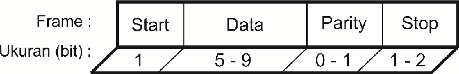
\includegraphics[width=1\textwidth]{figures/serialframe.png}}
	\caption{Serial Frame}
	\label{serialframe}
\end{figure}	
\subsection{Fungsi Baud Rate}
Baud rate dideteksi untuk mengetahui keluaran dari perangkat yang memerlukan basis serial untuk mengecek kecepatan data dan data itu sendiri. \cite{anderson1973method} Secara singkat, mendeteksi baud rate terdiri dari menentukan kecepatan transmisi dari perangkat yang mendapatkan sinyal karena perangkat penerima dapat dengan tepat mendecode sinyal dan mengkonversikannya ke perangkat. Baud rate memberitahu kecepatan data yang dapat dikirim melalui komunikasi serial. Dalam bps sendiri, berarti diketahui berapa kecepatan data yang dialirkan. Biasanya baud rate yang dipakai adalah 9600. Semakin besar baud rate yang dipakai, semakin tinggi kecepatan transfer data. Tetapi makin tinggi kecepatan maka makin beresiko mengalami error data. Untuk itu, disarankan untuk memakai baud rate standar atau dibawah 115.201.

\section{Framing Data}
Framing data adalah teknik penyusunan data untuk dikirim melalui komunikasi serial. Pada gambar , Data yang dikirim melalui komunikasi serial biasanya dari 5 sampai 9 bit. Pada arduino, data yang dipakai berukuran 8 bit. Urutan dari pengiriman data biasanya mengikuti endian tertentu. seperti pengiriman most-significant-bit atau least-significant-bit terlebih dahulu yang dikirim.

